\documentclass[11pt,a4paper]{article}
\usepackage[margin=2.5cm]{geometry}
\usepackage{graphicx}
\usepackage{booktabs}
\usepackage{amsmath}
\usepackage{placeins}
\usepackage[colorlinks=true,linkcolor=black,citecolor=blue,urlcolor=blue]{hyperref}

% thebibliography prints its own unnumbered "References" heading; the numbered
% \section{References} already provides it, so swallow the next starred heading
% once (star and title consumed together) and the sections after the
% bibliography keep the normal \section.
\makeatletter
\newcommand{\swallownextsectionstar}{%
  \let\originalsection\section
  \renewcommand{\section}{\@ifnextchar*{\swallowsectionstar}{\originalsection}}}
\def\swallowsectionstar*#1{\let\section\originalsection}
\makeatother

\title{\textbf{Distributed Matrix Multiplication on Shared Memory:\\
An Empirical Study of Thread-Count Scaling}\\
\vspace{0.2cm}
\Large Big Data --- Bachelor's Degree in Data Science and Engineering (ULPGC)}

\author{\textbf{Aythami Lorenzo} \\[0.1cm]
\small University of Las Palmas de Gran Canaria \\
\small Code \& Data: \url{https://github.com/aythamilorenzo/bigdata-individual-assignments}}
\date{October 2026}

\begin{document}

\maketitle

\begin{abstract}
{\small
We study the behavior of a distributed implementation of dense square matrix
multiplication using Apache Spark, and compare it against its sequential
baseline and its thread-pool parallel counterpart from the earlier
assignments: all three methods execute the same cache-blocked $i$-$k$-$j$
kernel (tile side 64, float64) and are element-wise identical. The
distributed method partitions $A$ by row blocks across $p$ Spark workers,
broadcasts $B$ and collects the result blocks; the thread-pool method
distributes the same tiles across $p$ prestarted threads. We perform an
analysis of end-to-end runtime with an explicit phase decomposition
(broadcast, job, driver-side assembly), speedup $S(p) = T_{\mathrm{seq}}/T_p$,
parallel efficiency $E(p) = S(p)/p$, framework overhead of Spark relative to
the thread pool, and peak memory (resident set and Java heap), across sizes
$n \in \{500, 1000, 1500, 2000, 3000, 4000\}$ and thread counts
$p \in \{1, 2, 4, 6, 8, 12, 24\}$ on a 6-core / 12-logical-processor CPU.
Our experiments provide a reproducible benchmark of one distributed
multiplication scheme across a variety of problem sizes and thread counts to
guide future research in performance analysis of data-intensive workloads.
Based on our experiments, we recommend the thread-pool method whenever both
are available on one machine, and distributed execution only when its
setup and communication costs are amortised or when the data no longer fits
one machine; extra threads beyond the physical cores return diminishing or
no additional benefit for any method.
}
\end{abstract}

\setcounter{tocdepth}{1}
{\small\tableofcontents}
\newpage

\section{Introduction and objective}
\label{sec:introduction}

Matrix multiplication is a canonical workload for studying how algorithms,
hardware and runtime overhead interact. Assignments 1 and 2 established the
behavior of basic and optimised \emph{sequential} implementations as $n$
grows, ending with a cache-blocked kernel as the fastest sequential method
for the largest sizes. Assignment 3 extended that validated kernel into
\textbf{parallel execution on shared memory} using a thread pool. This study
extends it in the direction required by the assignment:
\textbf{distributed execution using Apache Spark}, comparing the three
implementations of the \emph{same} algorithm, numeric type, storage layout
and input matrices while only the thread count varies, so the measured
effect is attributable to the execution framework and not to a change of
algorithm.

\paragraph{Research question.}
\emph{RQ:} how does the thread count $p$ affect the runtime, speedup,
efficiency, framework overhead and memory of a distributed shared-memory
multiplication as $n$ grows, when does distributed execution help relative
to thread-level parallelism, and when does adding threads stop helping on
this machine?

\section{Background}
\label{sec:background}

The baseline kernel multiplies two $n \times n$ row-major float64 matrices
with cache blocking on the $i$-$k$-$j$ loop order: work is organised in
$64 \times 64$ tiles so that a 32~KB tile of $B$ stays resident in the
core's private cache while it is reused. Total arithmetic work is $2n^3$
multiply--adds.

For $p$ workers the natural parallel decomposition partitions the output
rows (equivalently, the $i$-tiles) among workers: each worker accumulates a
disjoint set of rows of $C = AB$, reading $A$ and $B$ concurrently and never
writing another worker's rows. With $n/p$ rows per worker the idealised
model is $T_p = T_{\mathrm{seq}}/p + T_{\mathrm{overhead}}$, giving speedup
\begin{equation}
S(p) = \frac{T_{\mathrm{seq}}(n)}{T_p(n, p)}
\end{equation}
and efficiency
\begin{equation}
E(p) = \frac{S(p)}{p} \le 1 \quad \text{(ideal case)}.
\end{equation}
The overhead term $T_{\mathrm{overhead}}$ is method-dependent: the
thread-pool method pays task dispatch and join inside one address space,
while the Spark method additionally pays context setup, serialization of
the broadcast variable, per-task scheduling and result collection to the
driver. Separating these costs is one of the goals of this study.

\section{Methodology}
\label{sec:methodology}

\subsection{Implementations}

Three methods are written in Java 17 and perform the same arithmetic on the
same storage:
\begin{itemize}
    \item \texttt{blocked\_ijk\_sequential} --- the cache-blocked kernel of
    assignment 2 (block size 64), reused and validated by its test suite;
    the mandatory \emph{equivalent baseline}. It runs on the calling thread
    and always reports $p = 1$.
    \item \texttt{blocked\_ijk\_parallel} --- the same kernel's $i$-tiles
    partitioned across a fixed pool of $p$ prestarted threads (assignment 3,
    reused verbatim). Every output row has exactly one writer and the same
    ascending-$k$ accumulation order as the sequential kernel.
    \item \texttt{blocked\_ijk\_distributed} --- the same kernel's $i$-tiles
    partitioned across $p$ Spark workers: $A$ is partitioned by contiguous
    row blocks, $B$ is broadcast to all workers and the result blocks are
    collected to the driver. The workers run the same tile loops, so the
    result is element-wise identical to the other two methods.
\end{itemize}

\subsection{Workers, processes and machines}
\label{sec:workers}

Throughout this report, $p$ counts \emph{worker threads}. The distributed
method runs on Spark \texttt{local[$p$]}, which starts $p$ worker threads
inside a \emph{single JVM process} sharing one address space and one heap.
It does \emph{not} launch isolated worker JVM processes and does \emph{not}
span more than one physical machine: there is no network transfer, and the
``communication'' cost we measure is the serialization and copying of the
broadcast variable and the result blocks inside one process. A Spark
standalone cluster would run one worker process per machine and add real
network transfer; that configuration is outside the scope of this
assignment (local execution was explicitly permitted by the instructor) and
is discussed as a limitation. Consequently, the distributed-versus-thread
pool comparison isolates the \emph{framework} overhead of Spark
(scheduling, serialization, task lifecycle) from the algorithmic and
hardware effects, which are identical by construction.

\subsection{Inputs and environment}

The campaign multiplies the shared dense inputs of assignments 1 and 2
(little-endian float64, row-major, NumPy PCG64 seeded with $[42, n]$,
values uniform in $[0,1)$): sizes 500, 1000, 1500 and 2000 are
byte-identical to the assignment 2 inputs; $n = 3000$ and $n = 4000$ are
new and generated with the same generator and seed scheme. All three
methods of every configuration multiply the identical bytes.

Experiments ran inside WSL2 (Ubuntu) on an Intel Core i7-10750H (6 physical
cores, 12 logical processors, 2 threads per core) with 16~GB DDR4, affinity
mask \texttt{0-11}, OpenJDK 17.0.20.1, Maven 3.9.12, Apache Spark 3.5.1
and Python 3.14.4 (numpy 2.5.3, pandas 3.0.6, matplotlib 3.11.2). The
runner records these facts (\texttt{cpu\_model}, \texttt{physical\_cores},
\texttt{logical\_processors}, the affinity mask and the processor count
visible to the JVM) in its log for every configuration.

Thread counts $p \in \{1, 2, 4, 6, 8, 12, 24\}$ were chosen to cover the
mandatory single thread, the physical-core count (6), the logical-processor
count (12) and a deliberate $2\times$ \emph{oversubscription} (24), which is
identified as such throughout. The size range extends to $n = 4000$ (96~MB
per matrix, 288~MB for the three) so that the arithmetic work clearly
dominates the fixed framework costs; $n = 8000$ was excluded on purpose
because the sequential baseline needs roughly 230~s per multiplication,
exceeding the 60~s budget of the protocol.

\subsection{Measurement protocol}

The end-to-end timer surrounds exactly one multiplication call. For the
distributed method this is the sum of three driver-side phases: the
\emph{broadcast} of $B$ to the workers, the Spark \emph{job} (task
dispatch, worker-side tile computation and result transfer to the driver)
and the \emph{driver-side assembly} of the final matrix. The worker-side
compute time summed across tasks is also recorded, as a separate,
non-additive quantity (workers run concurrently inside the job stage, so
the sum can exceed the job wall clock). For the sequential and thread-pool
methods the whole cost sits in the computation column. Outside every timer:
input loading, the per-configuration setup (SparkContext or thread-pool
creation, measured separately in its own column), checksum computation and
warm-up calls. Only \texttt{System.nanoTime()} is used.

Each configuration runs 3 warm-up repetitions (recorded, excluded) then 7
measured repetitions in a dedicated JVM, so the peak-memory readings of one
configuration are not polluted by the others. Every raw sample is kept and
medians with interquartile ranges are reported. The budget is 60~s per
multiplication; an overrun would be recorded as a result, not a failure
(none occurred). Speedup and efficiency are computed from medians.

\subsection{Memory}

Two different quantities are recorded per configuration and never compared
as if identical: the process \emph{peak resident set size} read from
\texttt{/proc/self/status} (\texttt{VmHWM}) and the Java \emph{peak heap}
usage from \texttt{MemoryPoolMXBean}. The theoretical dense storage,
$24n^2$ bytes for the three matrices, is reported alongside as a reference
point; it is a lower bound on what any implementation needs.

\subsection{Correctness}

The three kernels are validated in-JUnit against each other on identity,
zero, known-answer $3 \times 3$ and seeded random matrices across sizes and
thread counts, including tests asserting that the checksum is invariant
with $p$ (14 tests). Independently, \texttt{correctness\_check.py} compares
jar checksums from all three methods against a NumPy float64 reference
($\mathrm{rtol} = 10^{-9}$, $\mathrm{atol} = 10^{-12}$).

\section{Results}
\label{sec:results}

The campaign produced 900 raw timing samples (6 sizes $\times$ 15
configurations $\times$ (3 warm-ups + 7 measured)) and 180 memory rows; all
checksums are identical across methods and thread counts at every size, as
the shared-kernel design predicts. All tables report the median of the 7
measured repetitions. The sequential baseline takes 64~ms at $n = 500$ and
26.7~s at $n = 4000$; every configuration completed within the 60~s budget.

\subsection{Runtime, speedup and efficiency}

The thread-pool method is faster than the Spark method in \emph{every}
measured cell of Table~\ref{tab:times}, and both distributed methods beat
the sequential baseline from $p = 2$ onwards at $n \ge 1000$. The best
measured speedups are $5.75\times$ for the thread pool ($n = 1500$,
$p = 12$) and $4.47\times$ for Spark ($n = 4000$, $p = 12$); no
configuration reaches the ideal $S(p) = p$ line
(Figure~\ref{fig:speedup}). At $n = 500$ Spark is \emph{slower than the
sequential baseline at every thread count} ($S \le 0.75$): the
multiplications are too short for the framework costs to amortise.

Efficiency (Figure~\ref{fig:efficiency}) is near-ideal for the thread pool
at $p = 2$ ($E = 0.86$--$0.94$), degrades to $0.66$--$0.76$ at the
physical-core count $p = 6$ and $0.46$--$0.48$ at $p = 12$, and collapses
to $0.18$--$0.24$ under oversubscription ($p = 24$). Spark's efficiency is
lower at every point ($E(p = 12) = 0.29$--$0.37$) because its overhead
term grows with the number of tasks. Increasing $p$ from 12 to 24 yields
no reliable gain for either method --- the $n = 2000$ thread-pool speedup
actually \emph{drops} from $5.56$ to $4.72$ --- as expected when 24
runnable threads time-share 12 hardware contexts.

\begin{table}[htbp]
\centering
\caption{Median end-to-end time per multiplication (milliseconds):
sequential baseline and the two distributed methods at each thread count.}
\label{tab:times}
\footnotesize
\begin{tabular}{rcccccccc}
\toprule
 & & \multicolumn{7}{c}{thread pool} \\
\cmidrule(lr){3-9}
$n$ & seq. & $p{=}1$ & $p{=}2$ & $p{=}4$ & $p{=}6$ & $p{=}8$ & $p{=}12$ & $p{=}24$ \\
\midrule
500  & 64 & 66 & 34 & 24 & 21 & 15 & 15 & 15 \\
1000 & 535 & 555 & 299 & 182 & 157 & 120 & 112 & 104 \\
1500 & 1644 & 1636 & 871 & 595 & 444 & 355 & 286 & 289 \\
2000 & 3317 & 3371 & 1939 & 1177 & 903 & 691 & 596 & 703 \\
3000 & 11260 & 11387 & 6400 & 3743 & 2829 & 2347 & 2005 & 2056 \\
4000 & 26734 & 27157 & 14843 & 8831 & 6709 & 5461 & 4867 & 4750 \\
\midrule
 & & \multicolumn{7}{c}{Spark local[$p$]} \\
\cmidrule(lr){3-9}
500  &  & 157 & 108 & 125 & 96 & 98 & 86 & 99 \\
1000 &  & 659 & 443 & 269 & 236 & 193 & 195 & 206 \\
1500 &  & 2006 & 1212 & 728 & 563 & 492 & 480 & 466 \\
2000 &  & 4850 & 2616 & 1636 & 1389 & 1042 & 933 & 974 \\
3000 &  & 15407 & 8609 & 4970 & 3629 & 3044 & 2596 & 2594 \\
4000 &  & 38259 & 19993 & 11379 & 8492 & 6970 & 5974 & 6392 \\
\bottomrule
\end{tabular}
\end{table}

\begin{table}[htbp]
\centering
\caption{Speedup $S(p) = T_{\mathrm{seq}}/T_p$ (upper blocks) and
efficiency $E(p) = S(p)/p$ (lower blocks), from medians.}
\label{tab:speedup}
\footnotesize
\begin{tabular}{rccccccc}
\toprule
$S(p)$ pool \textbackslash\ $p$ & 1 & 2 & 4 & 6 & 8 & 12 & 24 \\
\midrule
500  & 0.97 & 1.88 & 2.65 & 3.01 & 4.39 & 4.39 & 4.40 \\
1000 & 0.96 & 1.79 & 2.93 & 3.40 & 4.45 & 4.79 & 5.16 \\
1500 & 1.00 & 1.89 & 2.76 & 3.70 & 4.64 & 5.75 & 5.69 \\
2000 & 0.98 & 1.71 & 2.82 & 3.67 & 4.80 & 5.56 & 4.72 \\
3000 & 0.99 & 1.76 & 3.01 & 3.98 & 4.80 & 5.62 & 5.48 \\
4000 & 0.98 & 1.80 & 3.03 & 3.98 & 4.90 & 5.49 & 5.63 \\
\midrule
$S(p)$ Spark \textbackslash\ $p$ & 1 & 2 & 4 & 6 & 8 & 12 & 24 \\
\midrule
500  & 0.41 & 0.59 & 0.51 & 0.67 & 0.65 & 0.75 & 0.65 \\
1000 & 0.81 & 1.21 & 1.99 & 2.27 & 2.77 & 2.74 & 2.60 \\
1500 & 0.82 & 1.36 & 2.26 & 2.92 & 3.34 & 3.42 & 3.52 \\
2000 & 0.68 & 1.27 & 2.03 & 2.39 & 3.18 & 3.55 & 3.40 \\
3000 & 0.73 & 1.31 & 2.27 & 3.10 & 3.70 & 4.34 & 4.34 \\
4000 & 0.70 & 1.34 & 2.35 & 3.15 & 3.84 & 4.47 & 4.18 \\
\midrule
$E(p)$ pool \textbackslash\ $p$ & 1 & 2 & 4 & 6 & 8 & 12 & 24 \\
\midrule
500  & 0.97 & 0.94 & 0.66 & 0.50 & 0.55 & 0.37 & 0.18 \\
1000 & 0.96 & 0.89 & 0.73 & 0.57 & 0.56 & 0.40 & 0.22 \\
1500 & 1.00 & 0.94 & 0.69 & 0.62 & 0.58 & 0.48 & 0.24 \\
2000 & 0.98 & 0.86 & 0.70 & 0.61 & 0.60 & 0.46 & 0.20 \\
3000 & 0.99 & 0.88 & 0.75 & 0.66 & 0.60 & 0.47 & 0.23 \\
4000 & 0.98 & 0.90 & 0.76 & 0.66 & 0.61 & 0.46 & 0.23 \\
\midrule
$E(p)$ Spark \textbackslash\ $p$ & 1 & 2 & 4 & 6 & 8 & 12 & 24 \\
\midrule
500  & 0.41 & 0.30 & 0.13 & 0.11 & 0.08 & 0.06 & 0.03 \\
1000 & 0.81 & 0.60 & 0.50 & 0.38 & 0.35 & 0.23 & 0.11 \\
1500 & 0.82 & 0.68 & 0.56 & 0.49 & 0.42 & 0.29 & 0.15 \\
2000 & 0.68 & 0.63 & 0.51 & 0.40 & 0.40 & 0.30 & 0.14 \\
3000 & 0.73 & 0.65 & 0.57 & 0.52 & 0.46 & 0.36 & 0.18 \\
4000 & 0.70 & 0.67 & 0.59 & 0.52 & 0.48 & 0.37 & 0.17 \\
\bottomrule
\end{tabular}
\end{table}

\begin{figure}[htbp]
\centering
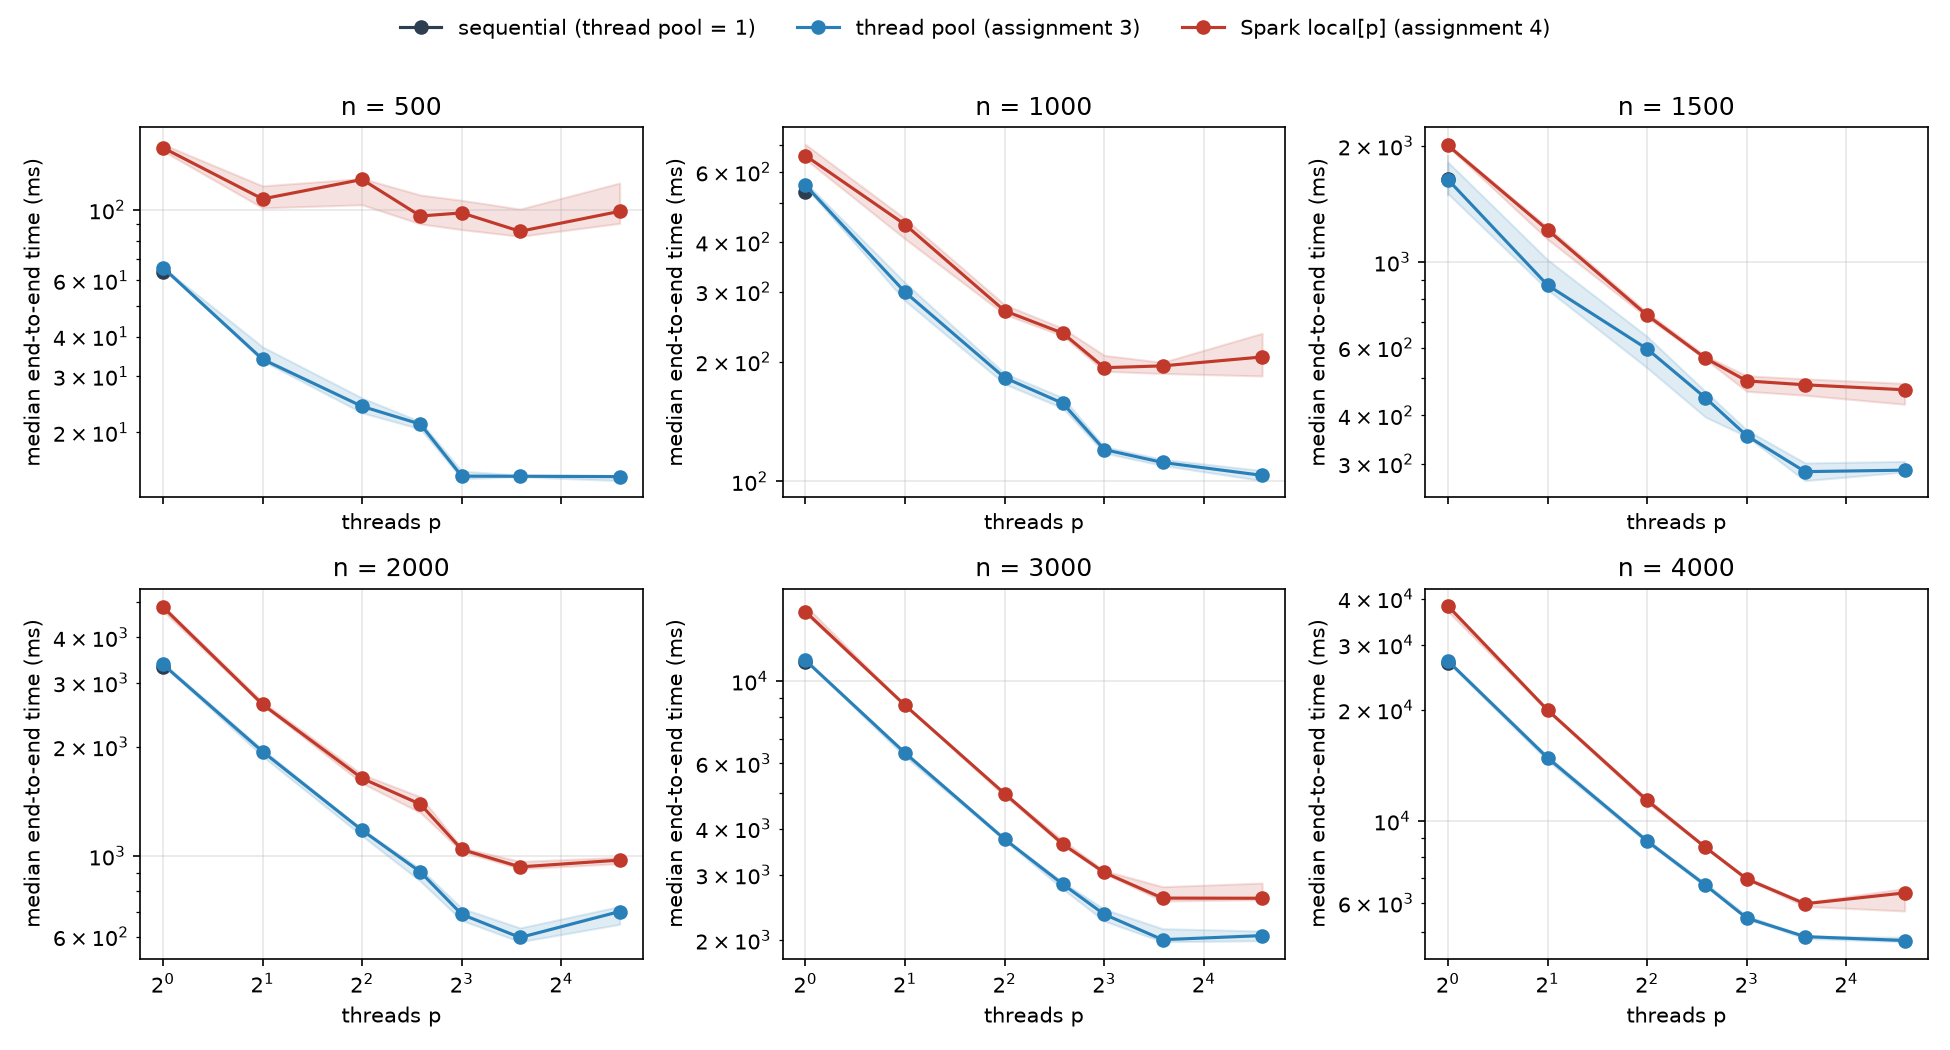
\includegraphics[width=0.72\linewidth]{figures/median_time_vs_threads.png}
\caption{Median end-to-end time per multiplication versus thread count
(log--log), per size; shaded bands are interquartile ranges.}
\label{fig:time}
\end{figure}

\begin{figure}[htbp]
\centering
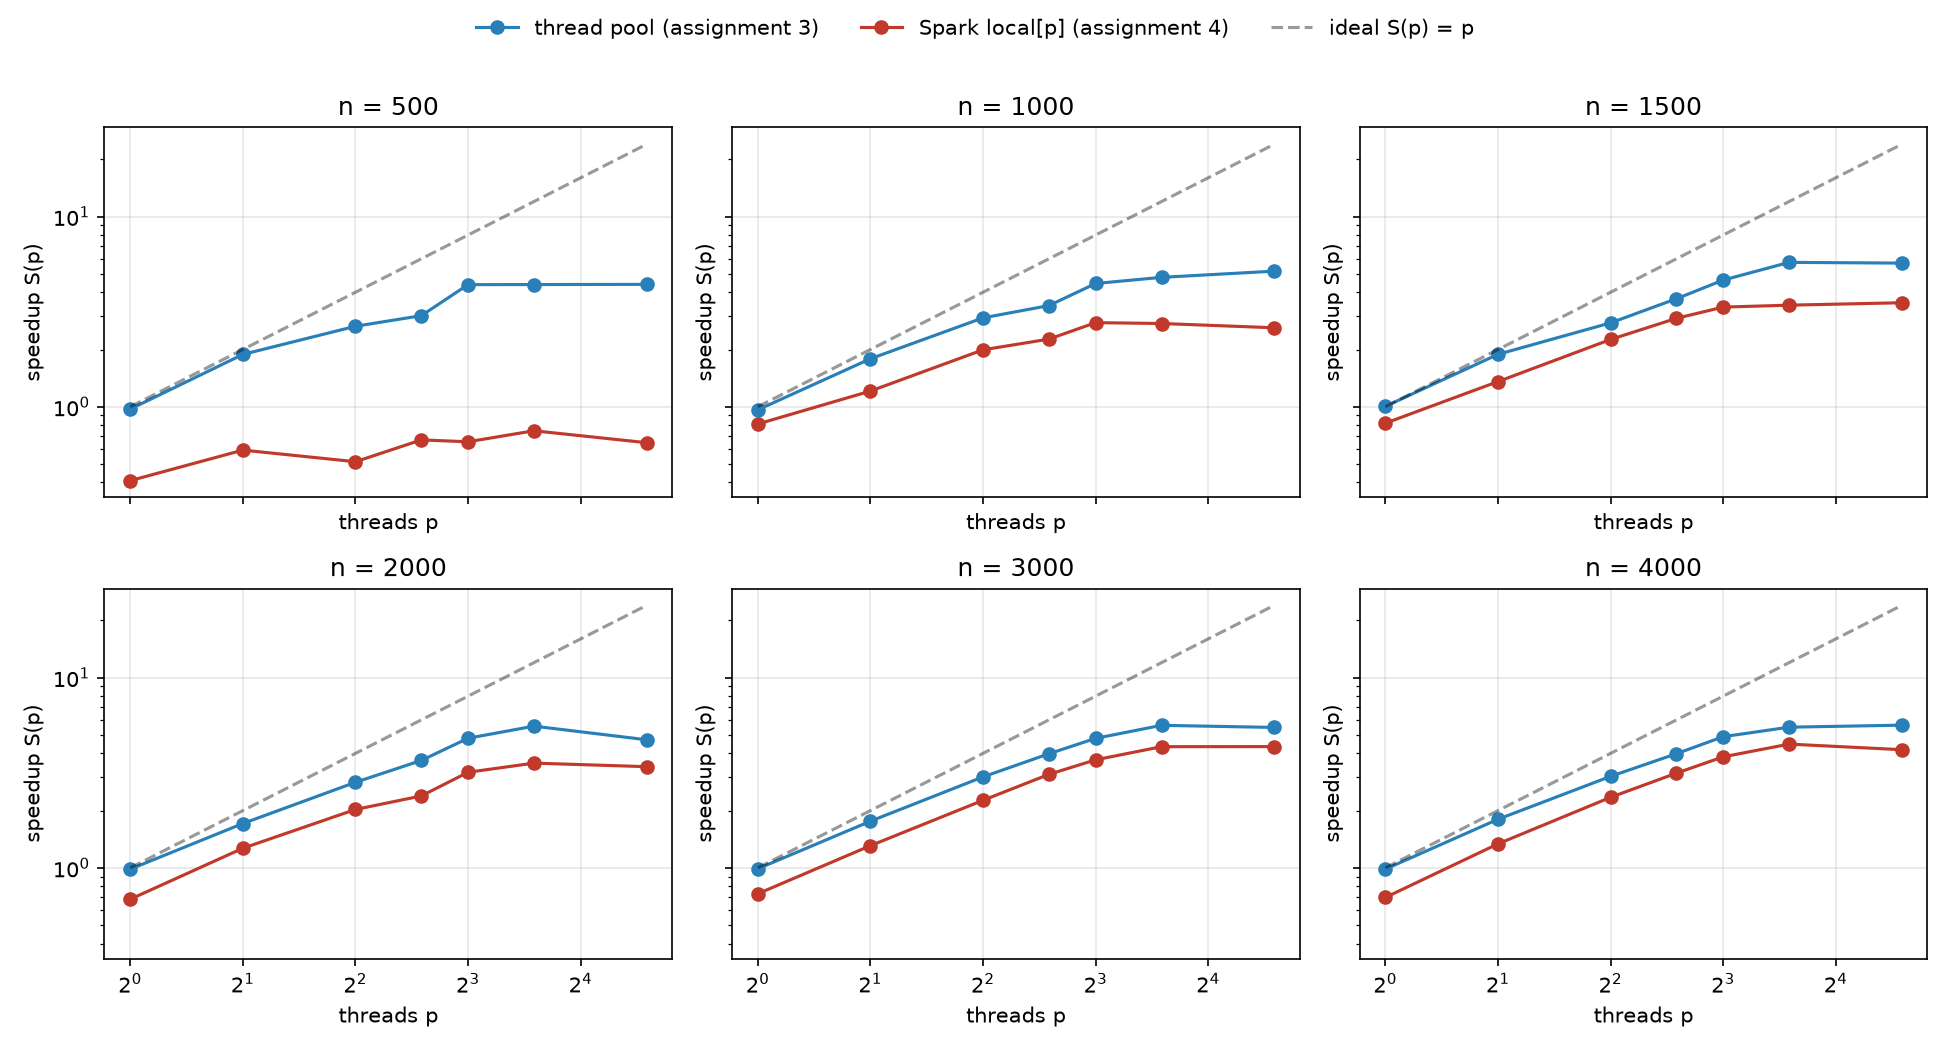
\includegraphics[width=0.72\linewidth]{figures/speedup_vs_threads.png}
\caption{Speedup $S(p) = T_{\mathrm{seq}}/T_p$ versus thread count for the
thread-pool and Spark methods, per size, against the ideal line
$S(p) = p$.}
\label{fig:speedup}
\end{figure}

\begin{figure}[htbp]
\centering
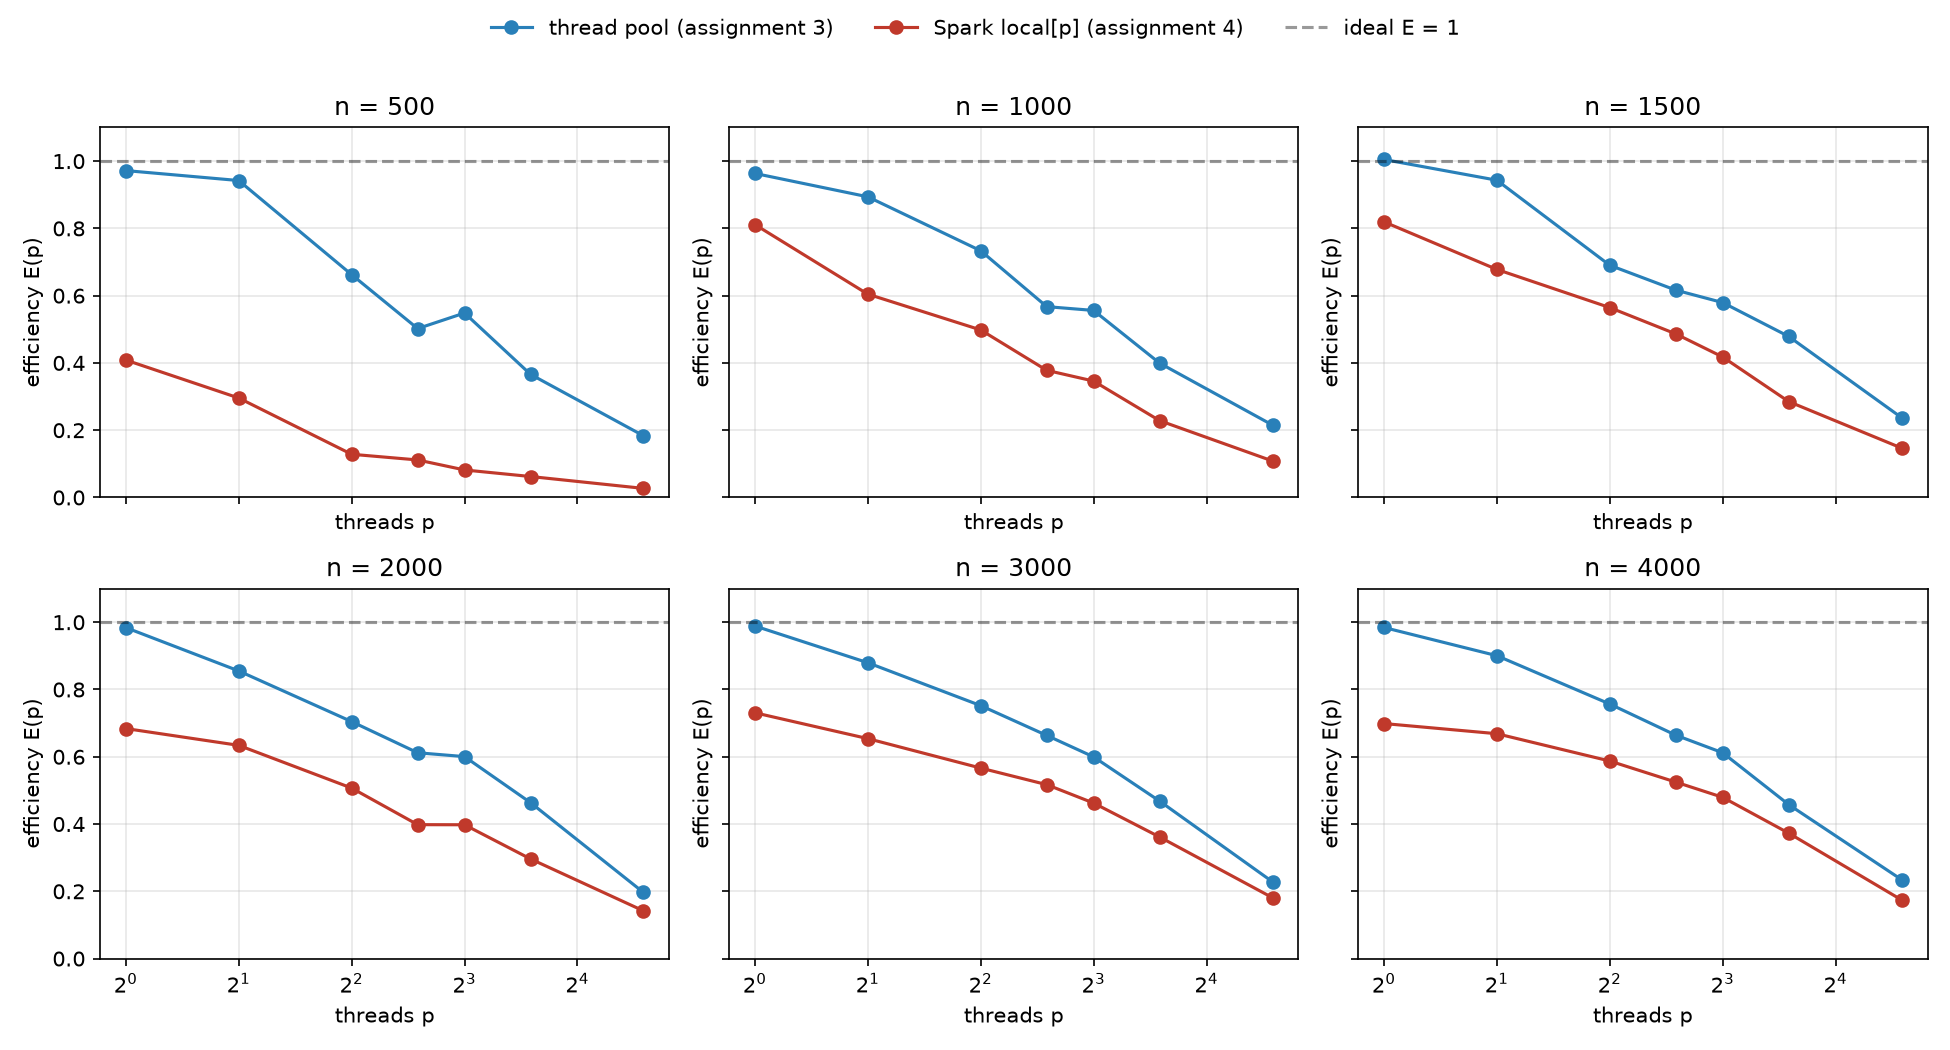
\includegraphics[width=0.72\linewidth]{figures/efficiency_vs_threads.png}
\caption{Parallel efficiency $E(p) = S(p)/p$ versus thread count, per size;
the dashed line marks the ideal $E = 1$.}
\label{fig:efficiency}
\end{figure}

\subsection{Framework overhead of Spark versus the thread pool}

Figure~\ref{fig:overhead} quantifies what the framework costs on top of the
identical kernel: the Spark method takes between $+23\%$ and $+41\%$ more
time than the thread pool at $n \ge 2000$, but the relative overhead grows
sharply as the problem shrinks ($+19\%$--$+98\%$ at $n = 1000$,
$+138\%$--$+580\%$ at $n = 500$). Two components explain the gap. First,
the per-call costs: Spark serializes each block of $A$ into the task
descriptor, deserializes it on the worker and ships the result rows back,
while the thread pool shares one address space and pays only dispatch and
join. Second, the per-configuration setup: creating the SparkContext takes
4.7--5.9~s (recorded separately), whereas the thread-pool constructor takes
about 10~ms; the setup alone exceeds every measured multiplication at
$n \le 1000$ and is only amortisable when many multiplications share one
context. At fixed $n$ the relative overhead is roughly flat in $p$ (23--35\%
at $n = 3000$--$4000$), so the framework cost scales with the data volume,
not with the number of workers.

\begin{figure}[htbp]
\centering
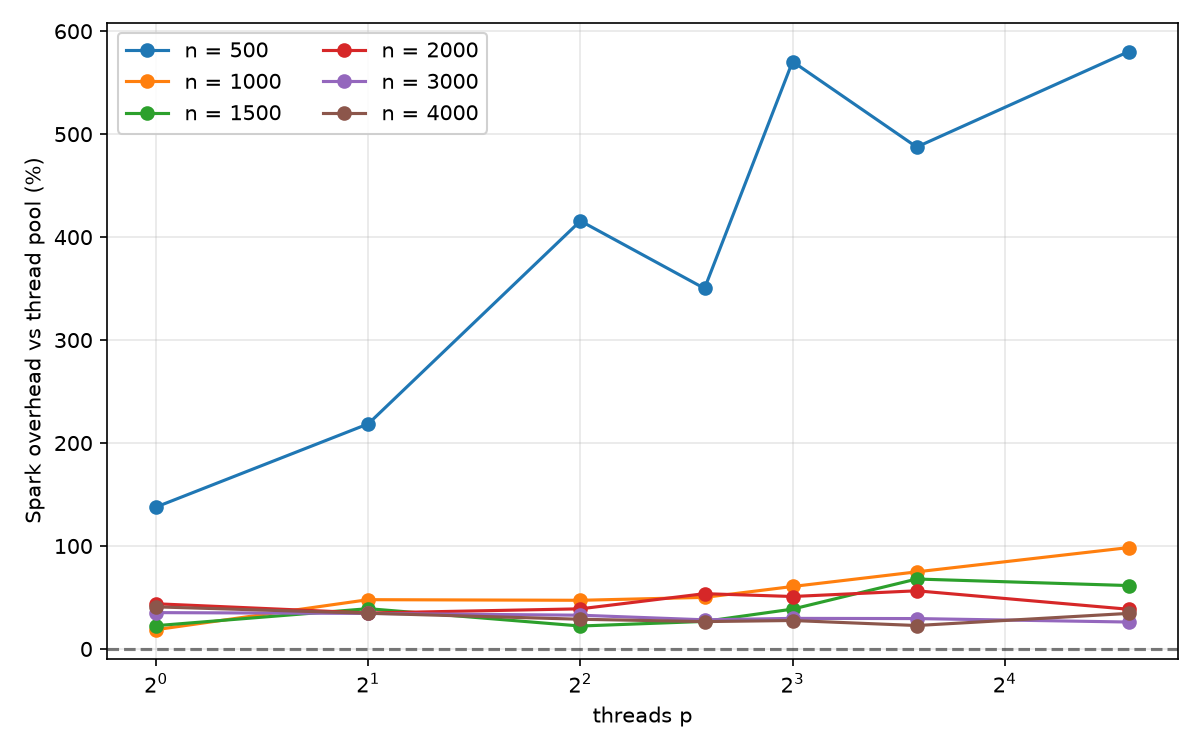
\includegraphics[width=0.72\linewidth]{figures/framework_overhead.png}
\caption{Spark overhead relative to the thread-pool method:
$T_{\mathrm{Spark}}(n,p)/T_{\mathrm{pool}}(n,p) - 1$, per size and thread
count.}
\label{fig:overhead}
\end{figure}

\subsection{Phase decomposition of the distributed method}

Figure~\ref{fig:breakdown} splits the Spark end-to-end time into the
broadcast of $B$, the job and the driver-side assembly. The broadcast
grows quadratically with $n$ --- 11~ms at $n = 500$, 220~ms at $n = 4000$,
matching the $8n^2$ bytes of $B$ --- but it is amortised by the
computation: it is 12\% of the end-to-end time at $n = 500$, $p = 12$ and
only 4\% at $n = 4000$, $p = 12$. The assembly of the final matrix is
negligible at all sizes (at most 59~ms, below 1\% for $n \ge 1000$). The
job dominates: it contains task scheduling, the tile loops and the
transfer of the result rows to the driver. Inside the job, the worker-side
compute time \emph{summed across workers} grows with $p$ even though each
worker's share shrinks: at $n = 4000$ the sum is 36.7~s at $p = 1$ but
132~s at $p = 24$ --- 3.6$\times$ more total CPU work for the same
arithmetic, evidence of memory-bandwidth and cache contention once the
physical cores are oversubscribed. This is why the summed column is
reported as a separate, non-additive quantity: the workers run
concurrently inside the job stage.

\begin{figure}[htbp]
\centering
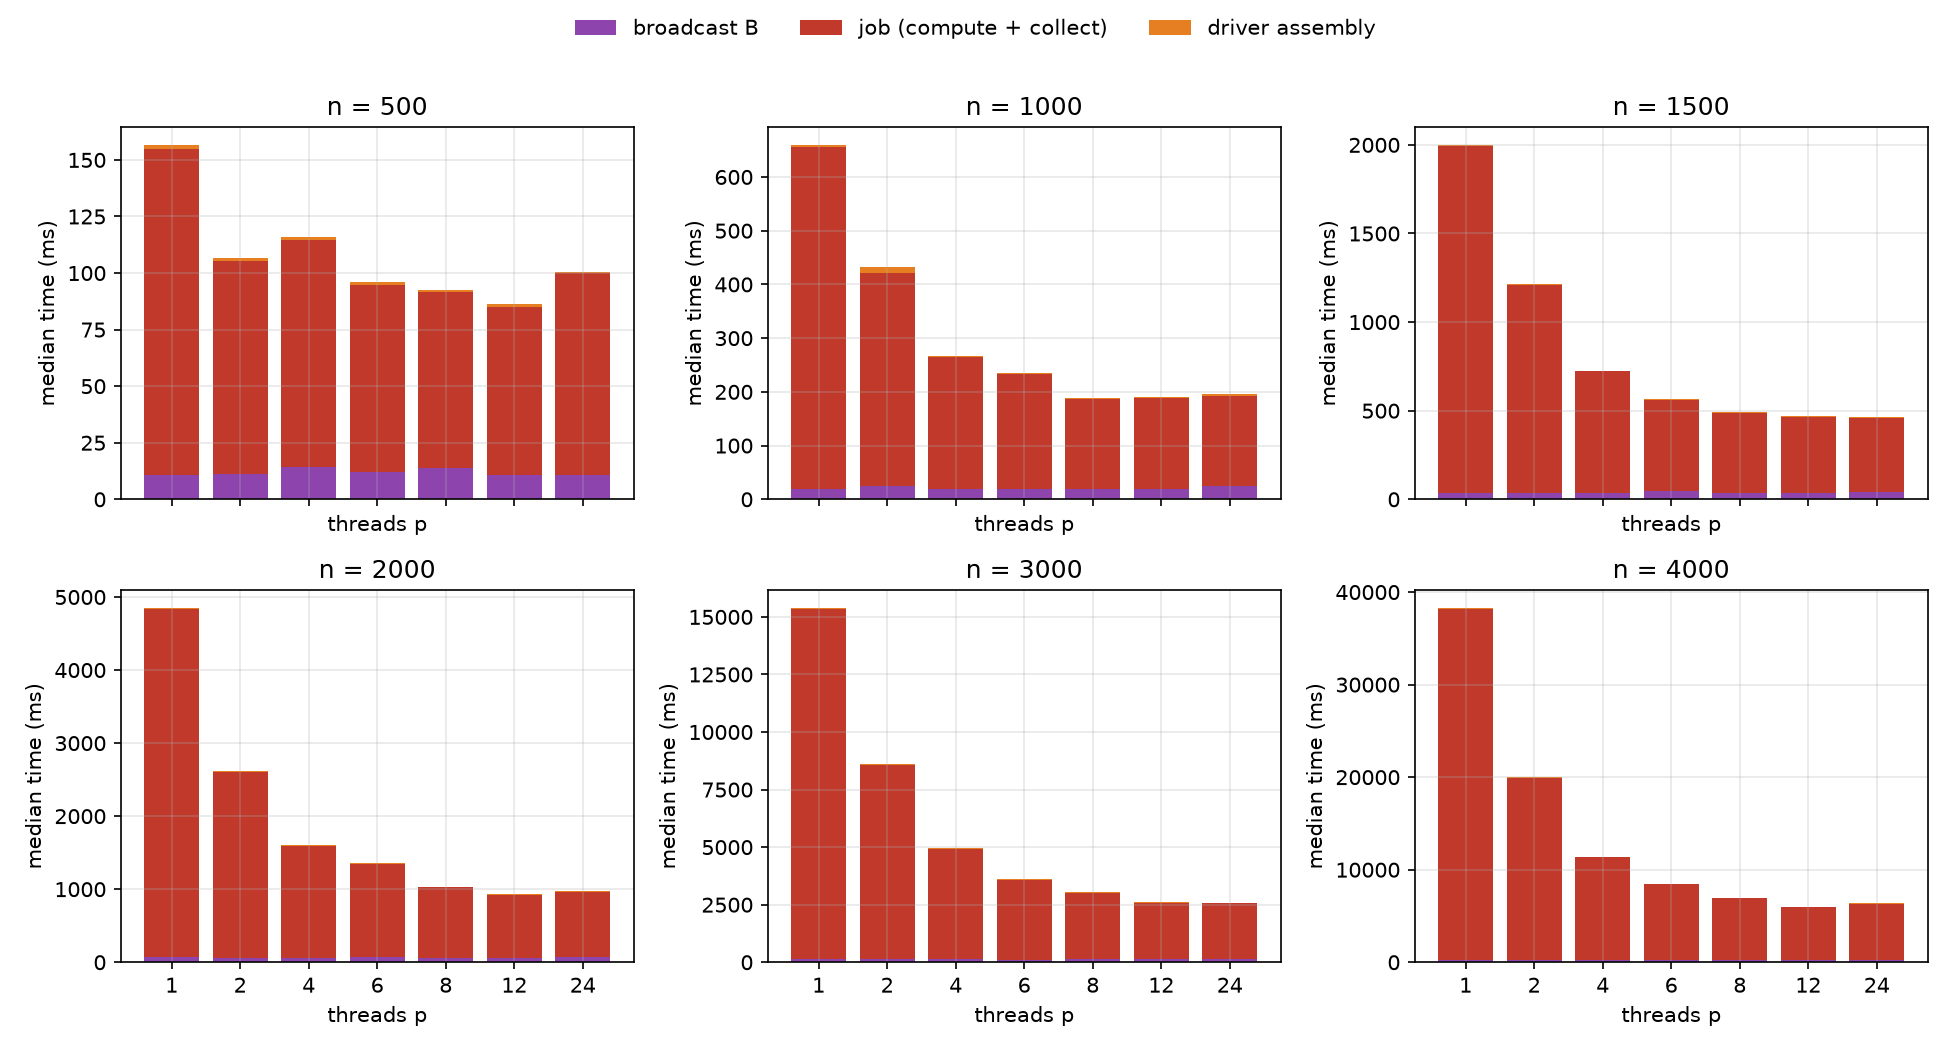
\includegraphics[width=0.72\linewidth]{figures/spark_phase_breakdown.png}
\caption{Phase decomposition of the Spark method's end-to-end time (medians,
stacked): broadcast of $B$, the Spark job and the driver-side assembly.}
\label{fig:breakdown}
\end{figure}

\subsection{Memory}

Peak memory (Figure~\ref{fig:memory}) separates the three families
clearly. The theoretical dense storage ($24n^2$ bytes) is 5.7~MiB at
$n = 500$ and 366~MiB at $n = 4000$. The sequential and thread-pool
methods sit near each other, 3--4$\times$ above the theoretical floor (JVM
runtime, loaded input buffers and the output matrix: 97~MiB at $n = 500$,
1.2--1.5~GiB at $n = 4000$), with the thread count barely moving the
needle. Spark pays a fixed framework floor of roughly 500~MiB even at
$n = 500$ (469--635~MiB RSS) and reaches 2.8--3.3~GiB at $n = 4000$
(7.8--9$\times$ the theoretical storage): on top of the same three
matrices it holds serialized task blocks of $A$, the broadcast copy of
$B$ and the collected result rows transiently. The peak heap follows the
same pattern (up to 2.7~GiB for Spark at $n = 4000$ versus 1.0~GiB for the
thread pool).

\begin{figure}[htbp]
\centering
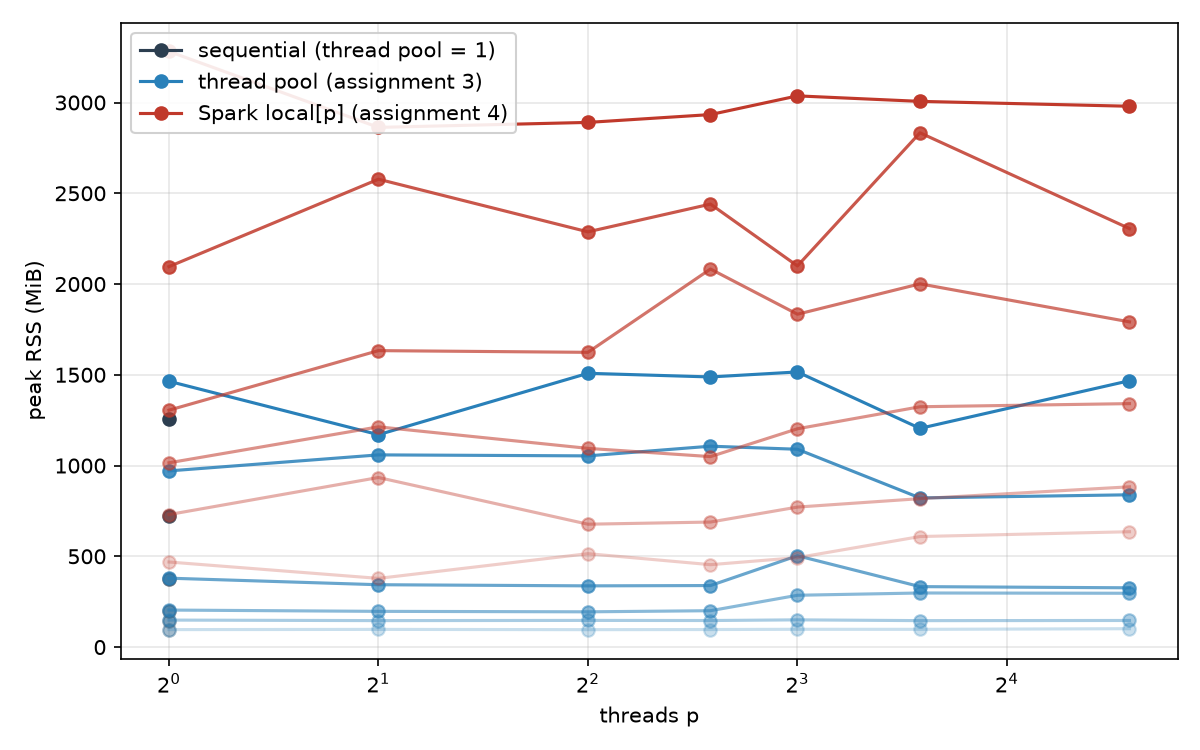
\includegraphics[width=0.72\linewidth]{figures/peak_rss_vs_threads.png}
\caption{Peak resident set size versus thread count, per size and method
(one line per size and method; darker shades are larger sizes).}
\label{fig:memory}
\end{figure}

\FloatBarrier
\section{Discussion}
\label{sec:discussion}

\paragraph{When does distributed execution help?}
The evidence answers the research question with three regimes.
\emph{First, thread-level parallelism dominates on a single machine:} the
thread pool beats Spark in all 42 paired cells (Table~\ref{tab:times}) and
reaches $5.75\times$ versus Spark's $4.47\times$ at best, because both
methods run the identical tile loops and the Spark method additionally
serializes task payloads, schedules jobs and collects results
(Figure~\ref{fig:overhead}). \emph{Second, the framework cost amortises
with problem size:} the Spark overhead falls from $+138$--$580\%$ at
$n = 500$ --- where Spark is slower than the single-threaded baseline at
every $p$ --- to $+23$--$41\%$ at $n = 3000$--$4000$, and the setup of
the SparkContext (4.7--5.9~s) becomes proportionally irrelevant. This is
the regime where distributed execution starts to make sense: large enough
data, many multiplications per context, or --- beyond the scope of this
single-machine study --- data that does not fit one machine or workers on
several machines. \emph{Third, adding workers stops helping at the
physical cores for both methods:} the thread pool peaks around
$p = 12$ ($E = 0.46$--$0.48$) and degrades at $p = 24$, and Spark shows
the same shape with lower plateaus ($E(12) = 0.29$--$0.37$). The
deliberate oversubscription ($p = 24$ on 12 hardware contexts) is never a
reliable win: at $n = 2000$ the thread-pool speedup drops from $5.56$ to
$4.72$ when going from $p = 12$ to $p = 24$.

\paragraph{Framework overhead, partitioning and hardware limits.}
The three effects can be separated with the decomposed timings. The
\emph{framework overhead} is the constant-ish gap between the two methods
(23--41\% at large $n$) plus the one-off context setup; it scales with
the data volume (serialization and broadcast of $B$, $8n^2$ bytes) but
only weakly with $p$. The \emph{partitioning granularity} is not a
limiting factor here: $n = 4000$ gives 63 row blocks of 64 rows, so the
24 tasks of the oversubscribed configuration still receive real work and
no partition is idle. The \emph{hardware limits} dominate the shape of
the curves: the summed worker compute time at $n = 4000$ grows from
36.7~s ($p = 1$) to 132~s ($p = 24$), 3.6$\times$ more total CPU time for
the same arithmetic, while wall time falls far less than proportionally
--- the signature of memory-bandwidth and cache contention once 12
hardware contexts are oversubscribed~\cite{hennessy2017}.

\paragraph{Non-monotonicities and variability.}
Speedup is not monotone in $p$ in both families: the $n = 500$ thread-pool
cells plateau at $\approx 4.4$ from $p = 8$ onwards (the multiplications
take 15~ms, so dispatch and scheduling noise is a visible fraction), and
the Spark curve at $n = 500$ oscillates within $S = 0.51$--$0.75$ without
a trend. Where the cells are long and stable ($n = 4000$: the $p = 12$
thread-pool cell has a 2.9\% IQR) the ordering is regular. No
configuration shows a superlinear speedup ($S(p) > p$ nowhere), so no
frequency-scaling or cache-residency explanation is required. One
implementation-level effect was measured and corrected during the
campaign: the first version of the Spark tasks captured the full matrix
$A$ in the task closure, which serialized 128~MB per task and exhausted
the 3~GB heap at $n = 4000$, $p = 24$; the final implementation sends
each task only its own rows of $A$, and all reported numbers come from
that version.

\subsection{Threats to validity}

Results are scoped to one machine, one JVM, one kernel (cache-blocked
$i$-$k$-$j$, tile 64, not tuned), the tested sizes ($n \le 4000$) and the
declared thread counts. The machine is a laptop: frequency scaling and
thermal behaviour affect the single-threaded baseline
($T_{\mathrm{seq}}$) and hence every ratio built on it. WSL2 adds a
virtualisation layer whose scheduling of the 12 logical processors is not
under the experimenter's control; the affinity mask was left at its default
(\texttt{0-11}) and recorded, not narrowed. Only one partitioning strategy
(contiguous row blocks) and one runtime mechanism (Spark
\texttt{local[$p$]}) were tested for the distributed family; no network
transfer and no multi-machine memory were exercised
(Section~\ref{sec:workers}), so the measured Spark overhead is a lower
bound on what a real cluster would add. The worker-side compute sum is
derived from in-task timers and includes the workers' view of the tile
loops only, not serialization.

\section{Conclusions}
\label{sec:conclusions}

\paragraph{Answers to the research question.}
(1) \emph{Thread-level parallelism is the right tool on a single machine:}
the thread-pool method is faster than the Spark method in every measured
cell and reaches a best speedup of $5.75\times$ ($n = 1500$, $p = 12$)
against Spark's $4.47\times$ ($n = 4000$, $p = 12$), both on the same
kernel with bit-identical results. (2) \emph{Distributed execution helps
against the sequential baseline only when the work per framework call is
large enough:} Spark beats the sequential baseline from $p = 2$ onwards
for $n \ge 1000$ ($S = 1.21$--$4.47$) but loses at $n = 500$ at every
thread count ($S \le 0.75$), where its fixed costs --- 4.7--5.9~s of
context setup plus 23--41\% per-call overhead --- dominate. (3)
\emph{Adding workers beyond the physical cores has sharply diminishing
returns for both methods:} efficiency at $p = 24$ falls to 0.18--0.24
(thread pool) and 0.03--0.18 (Spark), and the summed worker compute time
at $n = 4000$ inflates 3.6$\times$ from contention. (4) \emph{Memory
separates the methods more than time does:} Spark needs 2.8--3.3~GiB
resident at $n = 4000$ (7.8--9$\times$ the theoretical 366~MiB of
storage) versus 1.2--1.5~GiB for the thread pool and the sequential
baseline, because of serialized task payloads, the broadcast copy of $B$
and collected result rows.

\paragraph{Recommendation.}
On one machine with both options available, use the thread-pool method:
same results, 23--580\% less time, half the memory. Reach for Spark when
the data outgrows one machine or one address space, or when many
multiplications can share one long-lived context to amortise its setup;
then run with $p$ set to the physical cores (6 here) or at most the
logical processors (12), never oversubscribed. Keep $n \ge 1000$ for any
distributed run below which the framework, not the arithmetic, dominates.

\paragraph{What remains open.} Only one partitioning strategy (contiguous
row blocks) and one distributed runtime (Spark local mode) were tested;
real multi-machine execution with network transfer, work-stealing pools and
different tile sizes remain unexplored; memory-bandwidth saturation was not
measured directly (no hardware counters); and the vectorisation extension
of the assignment was declared not undertaken.


\section{References}
\swallownextsectionstar

\begin{thebibliography}{9}
    \bibitem{amdahl1967}
    G.~M. Amdahl, ``Validity of the single processor approach to achieving
    large scale computing capabilities,'' in \emph{Proc. AFIPS Spring Joint
    Computer Conference (SJCC)}, vol.~30, 1967, pp. 483--485.

    \bibitem{hill2008}
    M.~D. Hill and M.~R. Marty, ``Amdahl's law in the multicore era,''
    \emph{Computer}, vol.~41, no.~7, pp. 33--38, 2008.

    \bibitem{lam1991}
    M.~Lam, E.~E. Rothberg, and M.~D. Smith, ``The cache performance and
    optimizations of blocked algorithms,'' in \emph{Proc. 4th Int. Conf. on
    Architectural Support for Programming Languages and Operating Systems
    (ASPLOS)}, 1991, pp. 63--74.

    \bibitem{hennessy2017}
    J.~L. Hennessy and D.~A. Patterson, \emph{Computer Architecture: A
    Quantitative Approach}, 6th~ed. Morgan Kaufmann, 2017.

    \bibitem{spark2024}
    Apache Spark Team, \emph{Apache Spark Documentation}, 2024.
    \url{https://spark.apache.org/docs/latest/}
\end{thebibliography}

\section{Reproducibility materials}

All materials ship with this report: the Java (Maven) and Python sources;
the JUnit tests and the independent NumPy cross-check; the input
generator; the raw campaign CSVs and run log; and the figure script plus
figure PNGs. They are attached as the archive
\texttt{Assignment04\_}\allowbreak\texttt{Lorenzo\_}\allowbreak
\texttt{Materials.zip} to the \texttt{assignment-04}
release of the course repository. From the project root, inside WSL2:

{\footnotesize
\begin{verbatim}
.venv/bin/python python/generate_inputs.py
mvn -q verify
mvn -q -DskipTests package
.venv/bin/python python/correctness_check.py
.venv/bin/python python/run_experiments.py   # campaign
.venv/bin/python python/plot_results.py      # figures
\end{verbatim}
}

Exact toolchain versions and the full protocol are documented in
\texttt{README.md}. Runner exit codes: 0 (ok), 2 (invalid arguments), 3
(time budget exceeded), 4 (missing input files). The input binaries are
regenerated deterministically from seed 42 and are not shipped.
\url{https://github.com/aythamilorenzo/bigdata-individual-assignments}.\footnote{Generative AI
tools were utilized solely to refine the stylistic quality, grammar, and
technical phrasing of this report.}

\end{document}
